Method here, in past tense.

We reference like this using \verb|cleveref|: \cref{int:fig:example_a}, \cref{theo:eq:newton2}.

\subsection{Datasets}
    \comment{Here we describe how we construct and prepare the dataset. -\Carl}

    \subsubsection{MNIST}
        A simpler test for our neural networks is the MNIST benchmark dataset. It consists of 60 000 training images and 10 000 testing images. Each image consists $28 \times 28$ pixels depicting handwritten number between 0 and 9. As such, the images are to be classified to one of the 10 categories of digits. Some examples of the images in the dataset are depicted in \cref{met:fig:MNIST}.
        \begin{figure}
            \centering
            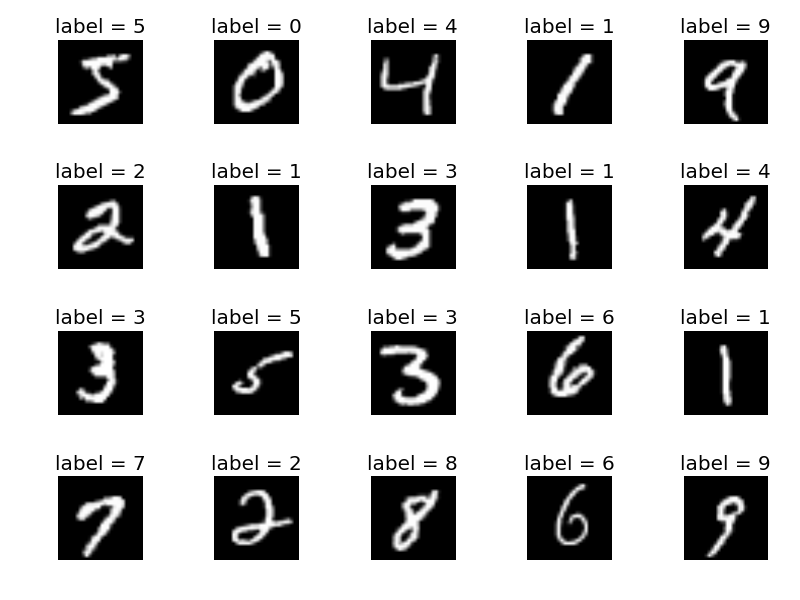
\includegraphics[width=\linewidth]{figs/MNIST_examples.png}
            \caption{20 example images from the MNIST dataset with their appropriate labels.}
            \label[fig]{met:fig:MNIST}
        \end{figure}

    \subsubsection{CIFAR-10}
        Initially, we applied our the LWTA NNs on the CIFAR-10 benchmark dataset for image recognition. This dataset consists of 60 000 images with $32 \times 32$ coloured pixels with RGB values, amounting to 3072 features per image. The images are divided into 10 categories, depicting one of either aeroplanes, birds, cars, cats, deer, dogs, frogs, horses, ships or trucks (see \cref{met:fig:CIFAR10}).

        \begin{figure}[ht!]
            \centering
            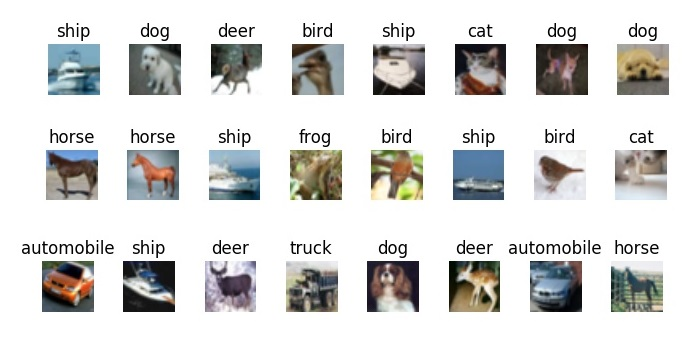
\includegraphics[width=\linewidth]{CIFAR10_examples.jpg}
            \caption{Examples of the images in the CIFAR10 dataset.}
            \label[fig]{met:fig:CIFAR10}
        \end{figure}

    \subsubsection{Premier League 2019 Season}
        \comment{The following is very draft-y. Will write it properly when my head is clear xD -\Nanna} 

        \comment{Maybe move some of this to intro? Not sure.}

        As well as for many other sports, data science is becoming more and more influential in the football industry~\citep{Herbinet2018}, both from the viewpoint of the club, e.g. in terms of choice of strategy or player acquisition and as seen by the odds market or the solely economically interested parties, be it e.g. club owners or league strategists, for making sure they benefit from the industry by possessing valuable data and powerful prediction algorithms. Analysts working in the larger leagues have access to technology that gives them more complex data than the main match events such as number of goals scored or corner given. For instance, a group on football analysts will most likely measure a team's or player's performance through metrics like expected goals (xG) or the number of passes allowed per defensive action (PPDA). The former is a very much used measure in football, but the algorithm behind it is not universal \comment{(entydig bestemt) -\Nanna}. In the European Premier League (EPL), one may follow live updates of the xG's for two opposing teams during their clash on several sites, however, the exact measurement will be dependent on the xG model the site uses.
        
        For the biggest football league in the world, the bookmakers tend to keep the most interesting data to themselves, as do the clubs' data science teams. However, being the most-watched football league in the world, the datasets form EPL are reliable and usually uncorrupted. 

        The challenges in collecting data and the time scope of this project compelled us to keep the purpose simple and ambitions somewhat low. In particular, we aim to foresee the outcome of a league match in EPL season 19/20 with a dataset as shown in \comment{some figure (work in progress)}. After preprocessing stats from various sources, our dataset contains information about $37\times 10$ league matches, but from the perspective of each team, giving $ 37 \times 10\times 2 = 740$ data points.
        
        The choice to look back only one league game for one team is due to a great ease in the data acquisition process. Trying to predict the full time result is a much more comprehensive task than to classify the outcome for a team as win (W), draw (D) or loss (L).


    \subsubsection{Data Preparation}
        \comment{Describe preprocessing of data, i.e. scaling etc. -\Carl}
        \comment{Data splitting \Anna}
        To train and evaluate our models we implemented the relevant data and as in our previous projects we split it in training data ($\sfrac{5}{6}$ of the data) and testing data ($\sfrac{1}{6}$ of the data) \citep{Project1, Project2}. When tuning the architecture, we further split the training data into a tuning set and a validation set used for monitoring overfitting, implementing early stopping with $p=5$. We used a split of $\sfrac{3}{4}$. See \cref{the:fig:illustration_data} for illustration of the data splitting. 

        \begin{figure}[]
            \centering
            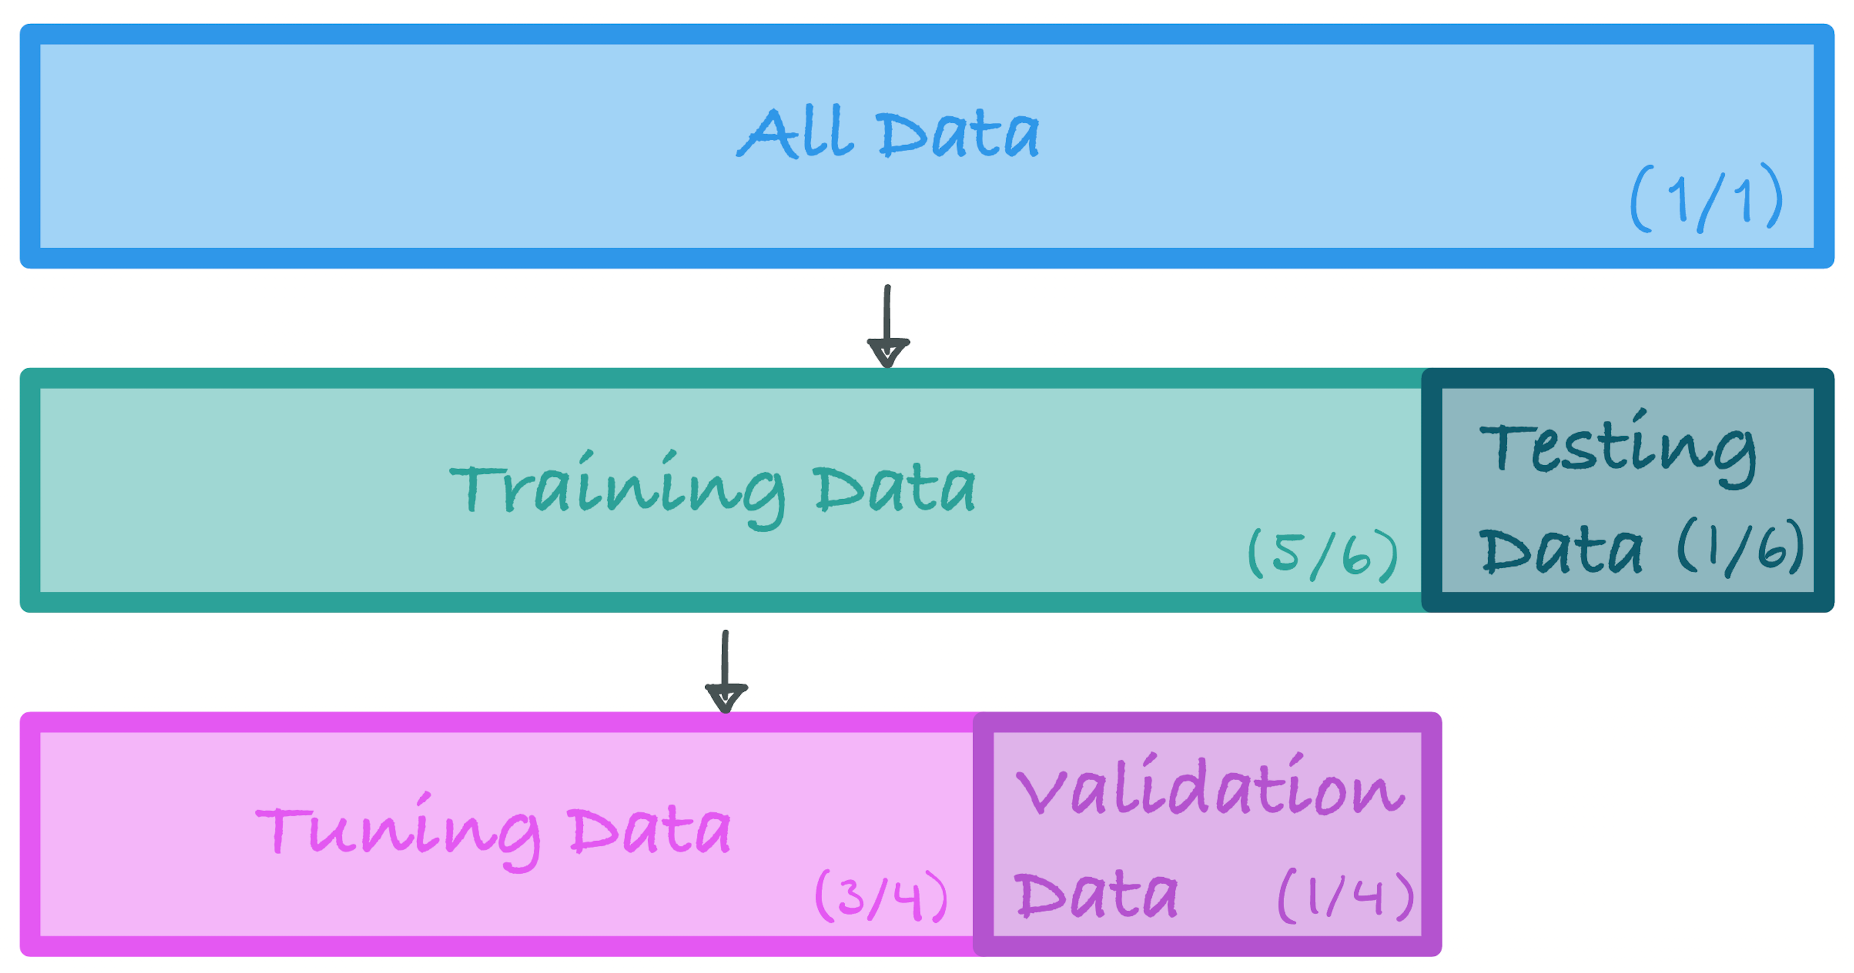
\includegraphics[width=.9\linewidth]{illustration_data.png}
            \caption{Illustration of data splitting.}
            \label[fig]{the:fig:illustration_data}
        \end{figure}

    \subsubsection{PCA}
        \comment{Could perhaps be part of data preparation \Anna} Before being subject to the principal component method, the Premier League data was z-score normalised, centring the mean around zero, with unit variance. This ensured that no single feature with a relatively large variance would dominate any of the principal components. The principal components found created a new basis for the data, and had similar shape as the original features (they were linear combinations of them). Extracting the first few of these yielded the most important components, used for further analysis. For all principal components we found the explained variance, which is the ``amount'' of variance accounded for by the principal component in question. In order to make an attempt at reducing the dimension of the problem, we found the number of principal components necessary in order to explain 99 \% of the variance of the original features \comment{Hmmm more/other/change idk \Johan}


\subsection{Neural Network training}

    \subsubsection{Initialisation of the Neural Network Weights}
        It is important to take care when initialising the weights and biases of a neural network to ensure fast convergence during training. We initialised the weights according to the He algorithm~\citep{He}. In our case it meant initialising the weights of node $i$ in layer $\ell$ by the distribution
        \begin{align}
            w^\ell_{ij} \distas \normal{0}{\sqrt{2/\hat{n}}},
        \end{align}
        where $\hat{n}$ is the number of inputs to the layer. The biases were all initialised to zero.

    \subsubsection{Optimisation Algorithm}
        When optimising the cost function of our problems we built on what we found in \citep{Project2}, using stochastic gradient descent with a batch size of 32. We used the Adam algorithm with hyperparameters $\beta_1 = 0.9$, $\beta_2 = 0.999$ and a learning rate $\eta = 0.001$. These hyperparameters were not tuned in any of our searches. The number of training epochs was decided with early stopping termination criterion. This means monitoring the loss of the network on a validation dataset after each epoch of training, and stopping the training if there is no improvement after a number of epochs $p$, called the \textit{patience}.

        All the datasets used pose classification problems with 3 or 10 categories. The cost function we used for optimisation was the standard categorical cross-entropy. Predicting probabilities $\vec{p}_c$ for the outcome being in category $c$ for the datapoints $\vec{y}_c$, with $n$ datapoints, the categorical cross-entropy is given by
        \begin{align}
            \mathcal{L}(\tilde{y}) = \sum_{i=1}^n \sum_{c \in \mathrm{categories}} y_{i,c} \log\pclosed{p_{i,c}}.
        \end{align}

        \comment{Discussion note: Early stopping prevents overfitting. -\Carl}

    \subsubsection{Regularisation}
        The first method we applied to combat overfitting was to add a L2 penalisation term to the kernel weights of the layers, as was done in \cite{Project2}. This adds a term to the cost function penalising large weights, and is parametrised with a hyperparameter $\lambda$, whose size is proportional to the penalisation.

        A problem that can occur in LWTA layers is when the weight of a certain input to one of the nodes of a group becomes much larger than those of the other nodes in the group, resulting in the output of the group being dominated by a single node and a single input. This can result in overly local training, perhaps even of a single node and a single weight. A common technique to combat this is to add a dropout layer before and/or after the LWTA layer. The dropout layer randomly sets elements of its input vector to zero, according to a dropout rate, before passing it on to the next layer. This means that the nodes in a group cannot solely lean on one specific node or input, and forces pathways in the network to not learn specific trends `too much'. As such, it prevents overfitting, and can be seen as a regularisation method. The dropout layers are only active during training, and do not drop any activations at inference time. The effect of dropout on a LWTA network is illustrated in \cref{met:fig:dropout_network}.

        \begin{figure}
            \centering
            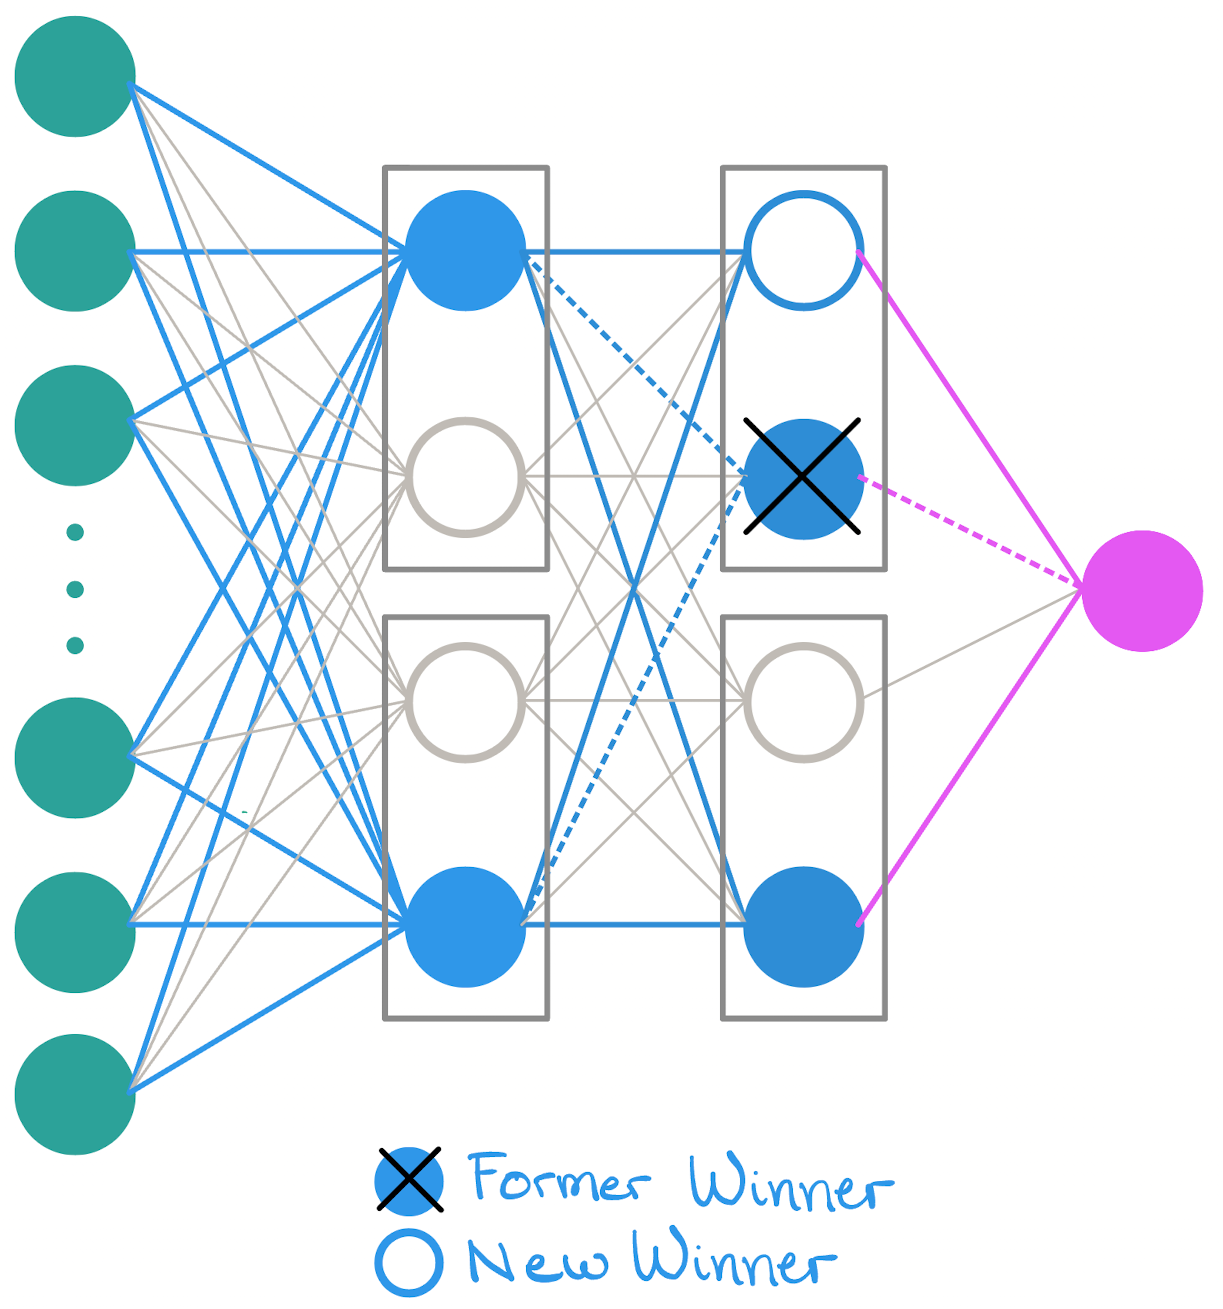
\includegraphics[width=.9\linewidth]{figs/illustration_dropout.png}
            \caption{An illustration channel-out neural network with a dropout added to the first channel-out layer. Only the lower group in the first hidden layer is trained.}
            \label[fig]{met:fig:dropout_network}
        \end{figure}

        When adding dropout to our networks, we did so with between every layer with the same dropout rate. This includes dropout on the input layer.


\subsection{Visualising Pathways}
    A good place to start with LWTA networks is to take a look at what actually happens during inference. We fitted a channel-out network on the full training MNIST dataset with three layers, 8 nodes in each and 4, 2 and 4 groups respectively in each network. This was done with a dropout rate of $0.125$, ridge penalisation added with $\lambda = 0.01$, and early stopping with $p=5$. We then plotted the pathways that were activated when inputting 200 test images depicting zeros, ones, fours and fives.

\subsection{Architecture tuning}
    To see what kind of network architectures were interesting and useful when applying to the datasets at hand, we tuned the architecture using the \textit{hyperband} search algorithm \citep{Hyperband}.

    We searched with a variable number of hidden layers between 2\textendash5, a number of nodes in the layers between 8\textendash64 in powers of 2, and a number of groups in the layers between 4\textendash32, again in powers of 2. When hyperparameters were chosen such that the number of groups was equal to or greater than the number of units in a layer, we set the layer to be a dense layer with the specified number of units, but added a ReLU activation to the output.

    \subsubsection{Hyperband Search}
        The hyperband search algorithm serves as a way to tune the hyperparameters of a model in a way such that more computing resources are dedicated to more promising areas of the hyperparameter space. It is based on the \textit{successive halving} algorithm, in which a finite budget $B$ (i.e. number of training epochs) is divided evenly between $n$ randomly sampled points from the hyperparameter space. These hyperparameters are then used to build $n$ models that are trained according to $r = B/n$ allocated resources on a tuning dataset, and their loss evaluated on a validation dataset, passing on the $k$ top performing models.\footnote{Usually the top half of the is passed on, as the algorithm name would indicate.} 
        These $k$ models are then trained further, with a new $n=k$ and consequently more resources $r$. This halving is then repeated until there is one model remaining. As hyperparameter points are discarded ($n$ decreases), the amount of allocated resources $r$ increases; meaning the more promising hyperparameter points are allotted exponentially more resources.

        This introduces a trade-off in the division of the resources $B$; sampling a larger number of hyperparameter points $n$ leaves less resources $r$ for exploring each point. The hyperband algorithm aims remedy this by doing a grid search of different values of $n$ and smaller resource allotments $r$. For each value of $n$ and $r$, the successive halving is performed, and the best preforming model is found. In the end, models that perform better deeper into the training will be found, but many hyperparameter points will have been explored.

        Hyperband takes two hyper(hyper)parameters, $R$ indicating the maximum amount of epochs of training for any single hyperparameter point, and a factor $\eta$ which is the reciprocal of the fraction of points that are passed on during each halving.

        \comment{$R=30$, $\eta=3$ gives $27+12+6+4 = 49$ hyperparameter points explored.}

        % \begin{algorithm}
        %     \caption{Hyperband search algorithm}
        %     \begin{algorithmic}[1]
        %         \Procedure{Hyperband}{$R, \eta$}
        %             \State $\msub{s}{max} \gets \floor{\log_\eta(R)},\quad B \gets (\msub{s}{max}+1) R$
        %             \For{$s \in \cclosed{\msub{s}{max}, \msub{s}{max}-1, \ldots, 0}$}
        %                 \State $n \gets \ceil{\frac{B}{R} \frac{\eta^s}{(s+1)}},\quad r \gets R\eta^{-s}$
        %                 \State $T \gets \mathtt{get\_hyperparameter\_configurations}(n)$
        %                 \For{$i \in \cclosed{0, \ldots, s}$}
        %                     \State $n_i \gets \floor{n \eta^{-i}},\quad r_i \gets r \eta^{i}$
        %                     \State $L \gets \cclosed{\mathtt{fit\_then\_eval\_val\_loss}(t, r_i): t\in T}$
        %                     \State $T \gets \mathtt{top\_k}(T, L, \floor{\sfrac{n_i}{\eta}})$
        %                 \EndFor
        %             \EndFor
        %         \EndProcedure
        %     \end{algorithmic}
        % \end{algorithm}

    \subsubsection{CIFAR-10}
        On the CIFAR-10 dataset, we tuned using 1 hyperband iteration with a maximum number of epochs $R=30$ and $\eta=3$. We used early stopping with $p=5$ to terminate the training. After finding best network architectures, we fitted them on the full training dataset, evaluating their accuracy on the test dataset. We used early stopping with $p=10$ during this training.

        When adding dropout we used a dropout rate of $0.1$, and with Ridge penalisation we used $\lambda=10^{-4}$.

    \subsubsection{Premier League Dataset}
        With the smaller Premier League dataset, we could afford 3 full iterations of the hyperband search with a maximum number of epochs $R=150$ and again $\eta=3$. Again, we used early stopping during the tuning, with $p=15$. After finding the top-performing architectures, we trained on the full training set with early stopping with $p=30$.

        When adding dropout we used a dropout rate of $0.25$, and with Ridge penalisation we used $\lambda=10^{-4}$.
